\documentclass[a4paper,12pt]{article}
\usepackage[utf8]{vietnam}
\usepackage[left=2.5cm,right=2.5cm,top=2.5cm,bottom=2.5cm]{geometry}
\usepackage{graphicx}
\usepackage{tocloft}
\usepackage{hyperref}
\usepackage{array}
\usepackage{longtable}
\usepackage[most]{tcolorbox}
\usepackage{setspace}
\usepackage{multicol}
\usepackage{lipsum}
\usepackage[table]{xcolor}

\geometry{a4paper, margin=1in}

\begin{document}

\begin{center}
\tcbset{
  colframe=green!60!black, % viền xanh lá đậm
  arc=5mm,              % bo tròn góc
  boxrule=1pt,          % độ dày đường viền
  width=1\textwidth,  % độ rộng khung
  enhanced,             % cho phép nhiều tính năng mở rộng
  center title,
  sharp corners=all,
  boxsep=10pt           % khoảng cách nội dung và viền
}

\begin{tcolorbox}
\begin{center}
\textbf{TRƯỜNG ĐẠI HỌC GIAO THÔNG VẬN TẢI TPHCM} \\[1.2em]

\textbf{VIỆN CÔNG NGHỆ THÔNG TIN VÀ ĐIỆN, ĐIỆN TỬ} \\[2em]

\includegraphics[width=0.8\textwidth]{uth.png} \\[2em]

\textbf{MÔN HỌC: LẬP TRÌNH THIẾT BỊ DI ĐỘNG} \\[1.5em]

\textbf{ĐỀ TÀI: APP TAKENOTE} \\[1.5em]

\textbf{Giảng viên:} Trương Quang Tuấn \\[1.2em]

\textbf{Nhóm thực hiện:} Nhóm 15 \\[1.2em]

\textbf{Thành viên:} \\[1.2em]

Trần Gia Huy \hfill MS: 079205047045 \\[0.8em]

Trương Quang Huy \hfill MS: 079205004440 \\[0.8em]

Nguyễn Hữu Đăng \hfill MS: 083205003614 \\[1.5em]

\textbf{Ngành:} Công nghệ thông tin \\[2em]

\textbf{THÀNH PHỐ HỒ CHÍ MINH, NĂM 2025}
\end{center}
\end{tcolorbox}
\end{center}

\clearpage

\tableofcontents

\clearpage

\section{LỜI MỞ ĐẦU}
Trong bối cảnh công việc ngày càng nhiều, nhu cầu ghi nhớ và note lại nhiệm vụ công việc ngày càng gia tăng thì app \textbf{TakeNote} xuất hiện như là cách để thay thế những ghi chú bằng tay. Điều này không chỉ giúp người dùng có thể thoải mái trong việc lưu giữ kiến thức, nhiệm vụ thiết yếu hằng ngày mà còn giảm số lượng rác thải từ việc sản xuất giấy phục vụ cho việc \textit{takenote} của người dùng.

Hệ thống \textit{TakeNote} nhằm mục đích giải quyết những khó khăn đó, giúp tối ưu hóa thời gian và đảm bảo tính chính xác, nâng cao chất lượng người dùng và mang đến trải nghiệm tốt nhất cho người sử dụng.

Trong bài báo cáo này, chúng em sẽ trình bày quá trình thiết kế và triển khai hệ thống app \textbf{TakeNote}. Nội dung bao gồm phân tích yêu cầu thực tế, thiết kế giải pháp kỹ thuật, triển khai hệ thống và đánh giá hiệu quả với nhu cầu người dùng mà còn mang lại giá trị bền vững trong quá trình hoạt động.

Hy vọng bài báo cáo sẽ cung cấp những thông tin hữu ích, đồng thời góp phần vào sự phát triển và đổi mới trong hệ thống app \textbf{TakeNote} này.

\section{KHẢO SÁT HIỆN TRẠNG VÀ YÊU CẦU HỆ THỐNG}
\subsection{Khảo sát}
\subsubsection{Giới thiệu sơ bộ về hệ thống}
Mục đích của hệ thống \textbf{TakeNote} là hỗ trợ người dùng trong việc ghi chú, tổ chức thông tin cá nhân một cách khoa học, nhanh chóng và tiện lợi. Hệ thống hướng đến việc tối ưu hóa quá trình tạo, quản lý và truy xuất ghi chú trên thiết bị di động, đồng thời nâng cao hiệu suất cá nhân và giảm thiểu các sai sót trong quá trình ghi chép thủ công. Thông qua giao diện thân thiện và dễ sử dụng, người dùng có thể dễ dàng lưu lại các ý tưởng, công việc cần làm, lịch trình hoặc bất kỳ thông tin nào cần thiết trong cuộc sống hằng ngày.

Ứng dụng \textbf{TakeNote} tích hợp các công nghệ hiện đại như \textit{Firebase Authentication}, \textit{Jetpack Compose}, và kiến trúc \textit{MVVM}, nhằm đảm bảo hệ thống hoạt động ổn định, bảo mật thông tin người dùng, và có khả năng mở rộng trong tương lai. Việc phân chia rõ ràng giữa giao diện, xử lý logic và dữ liệu không chỉ giúp dễ dàng phát triển và bảo trì hệ thống, mà còn tạo nền tảng vững chắc để phát triển các tính năng nâng cao như đồng bộ hóa ghi chú trên nhiều thiết bị hay phân loại thông minh.

Lợi ích của hệ thống bao gồm tự động hóa và tối ưu hóa việc ghi chú, giúp người dùng tiết kiệm thời gian, tránh bỏ sót thông tin quan trọng và tăng cường hiệu suất công việc cá nhân. Đồng thời, hệ thống hỗ trợ lưu trữ dữ liệu gắn với tài khoản người dùng, đảm bảo tính riêng tư và khả năng truy cập mọi lúc, mọi nơi. Giao diện được thiết kế tối giản nhưng hiện đại, dễ tiếp cận với mọi đối tượng người dùng, từ sinh viên, nhân viên văn phòng đến người dùng phổ thông.

Việc áp dụng công nghệ mới vào hệ thống không chỉ mang lại trải nghiệm người dùng mượt mà hơn mà còn thể hiện tính linh hoạt và thích nghi cao với nhu cầu thay đổi của người dùng. Qua đó, hệ thống \textbf{TakeNote} không chỉ là một ứng dụng ghi chú đơn thuần, mà còn là một công cụ hỗ trợ quản lý thông tin cá nhân hiệu quả, góp phần nâng cao chất lượng cuộc sống và hiệu quả làm việc của người dùng.

\subsubsection{Đánh giá hiện trạng}
\textbf{a) Ưu điểm:} Ứng dụng ghi chú hiện đại với giao diện đơn giản, dễ sử dụng, kết hợp kiến trúc \textit{MVVM}, \textit{Firebase Authentication} và \textit{Jetpack Compose} để tối ưu trải nghiệm người dùng. Ứng dụng cho phép tạo, chỉnh sửa, tìm kiếm và lưu trữ ghi chú nhanh chóng, bảo mật cao, hỗ trợ lưu trữ cục bộ và có khả năng mở rộng lên đám mây. Nhờ thiết kế trực quan, điều hướng linh hoạt và khả năng tích hợp nhiều tính năng nâng cao, \textbf{TakeNote} giúp nâng cao hiệu suất cá nhân và đáp ứng linh hoạt nhu cầu ghi chú mọi lúc, mọi nơi.

\textbf{b) Nhược điểm:} Do nhu cầu ghi chú ngày càng cao và sự phụ thuộc vào các ứng dụng \textit{TakeNote} để tổ chức công việc, học tập nên hiện nay các ứng dụng ghi chú vẫn tồn tại một số nhược điểm như:

\textbf{Khó kiểm soát lỗi và mất dữ liệu:} Nếu không có tính năng đồng bộ tốt hoặc sao lưu định kỳ, người dùng dễ gặp tình trạng mất ghi chú do lỗi ứng dụng hoặc thiết bị.

\textbf{Yêu cầu học cách sử dụng:} Một số ứng dụng có giao diện phức tạp, tính năng dày đặc, khiến người dùng mới mất thời gian để làm quen và sử dụng hiệu quả.

\textbf{Phụ thuộc vào kết nối Internet:} Nhiều ứng dụng chỉ hoạt động ổn định khi có mạng, đặc biệt là các ứng dụng có đồng bộ đám mây, gây khó khăn khi sử dụng ngoại tuyến.

\subsection{Mục tiêu của hệ thống}
\subsubsection{Yêu cầu chức năng}
\textbf{- Chức năng đăng nhập:} App cho phép người dùng tạo tài khoản bằng email và mật khẩu, xác thực người dùng qua \textit{Firebase Authentication}, hỗ trợ đăng nhập lại tự động nếu tài khoản đã được xác minh.

\textbf{- Tạo ghi chú:} Người dùng có thể tạo ghi chú mới với tiêu đề và nội dung, giao diện ghi chú hiển thị tiêu đề, nội dung rút gọn và thời gian cập nhật, giao diện cho phép cuộn mượt, hỗ trợ thao tác chạm để xem chi tiết.

\textbf{- Chỉnh sửa và xóa ghi chú:} Cho phép người dùng sửa nội dung ghi chú đã tạo, hỗ trợ xóa ghi chú khi không cần thiết, xác nhận trước khi xóa để tránh thao tác nhầm.

\textbf{- Giao diện người dùng (UI/UX):} Giao diện thiết kế bằng \textit{Jetpack Compose}, đơn giản, hiện đại và dễ sử dụng, tương thích tốt trên nhiều kích thước màn hình, màu sắc và bố cục dễ nhìn, hỗ trợ chế độ tối (\textit{dark mode}).

\subsubsection{Yêu cầu phi chức năng}
\textbf{- Tính hiệu năng:} Ứng dụng phải phản hồi nhanh, thao tác tạo, chỉnh sửa và xóa ghi chú được xử lý tức thì, không gây trễ đáng kể, hiển thị danh sách ghi chú mượt mà, hỗ trợ cuộn không giật lag kể cả khi có số lượng ghi chú lớn.

\textbf{- Tính bảo mật (Security):} Tài khoản người dùng được bảo vệ bằng xác thực \textit{Firebase Authentication}, tránh truy cập trái phép. Dữ liệu ghi chú cá nhân chỉ được truy cập bởi đúng người dùng đã đăng nhập.

\textbf{- Khả năng mở rộng (Scalability):} Hệ thống được thiết kế linh hoạt để dễ dàng tích hợp các tính năng mới trong tương lai như: nhắc lịch, gắn thẻ, ghi chú có hình ảnh, đồng bộ đám mây, v.v. Có thể mở rộng từ lưu trữ cục bộ sang lưu trữ và đồng bộ hóa bằng \textit{Firebase Firestore} mà không cần thay đổi cấu trúc lõi.

\textbf{- Tính khả dụng (Usability):} Giao diện đơn giản, trực quan, dễ tiếp cận cho người dùng mới.

\textbf{- Khả năng tương thích (Compatibility):} Hoạt động tốt trên các thiết bị Android từ phiên bản Android 8.0 (API 26) trở lên. Tương thích với cả điện thoại màn hình nhỏ và máy tính bảng.

\textbf{- Tính ổn định và bảo trì (Maintainability):} Mã nguồn được tổ chức rõ ràng theo kiến trúc \textit{MVVM}, dễ bảo trì và nâng cấp. Sử dụng các thư viện chính thức và được hỗ trợ lâu dài như \textit{Jetpack}, \textit{Firebase} để đảm bảo độ ổn định. Có thể kiểm thử các thành phần riêng biệt (\textit{unit test}, \textit{UI test}) để phát hiện và sửa lỗi dễ dàng.

\subsubsection{Mô hình hóa yêu cầu}
\begin{longtable}{|>{\raggedright}p{3cm}|>{\raggedright}p{4cm}|>{\raggedright}p{7cm}|}
\hline
\textbf{Actor} & \textbf{Use Case} & \textbf{Mô tả} \\ \hline
Người dùng & Đăng nhập & Cho phép người dùng đăng nhập vào hệ thống. \\ \hline
& Đăng ký tài khoản & Người dùng tạo tài khoản mới bằng email và mật khẩu \\ \hline
& Tạo ghi chú & Tạo mới một ghi chú gồm tiêu đề và nội dung \\ \hline
& Xem danh sách ghi chú & Hiển thị toàn bộ ghi chú đã lưu dưới dạng danh sách \\ \hline
& Xem chi tiết ghi chú & Xem nội dung đầy đủ của một ghi chú \\ \hline
& Chỉnh sửa ghi chú & Thay đổi nội dung ghi chú đã tạo \\ \hline
& Xóa ghi chú & Xóa bỏ ghi chú không còn cần thiết \\ \hline
& Tìm kiếm ghi chú & Tìm ghi chú không còn cần thiết \\ \hline
& Đăng xuất & Thoát khỏi tài khoản hiện tại \\ \hline
& Theme & Đổi màu sắc của layout trên app \\ \hline
\end{longtable}

\section{PHÂN TÍCH HỆ THỐNG}
\subsection{Sơ đồ Usecase tổng quan}
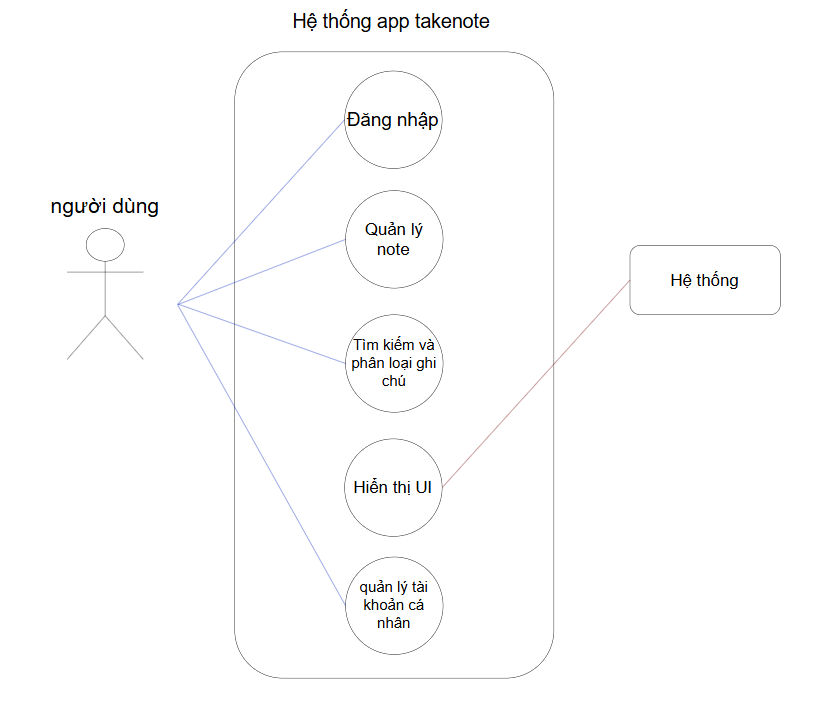
\includegraphics[width=0.8\textwidth]{useCaseTongQuan.png}
\subsubsection{Usecase đăng nhập}
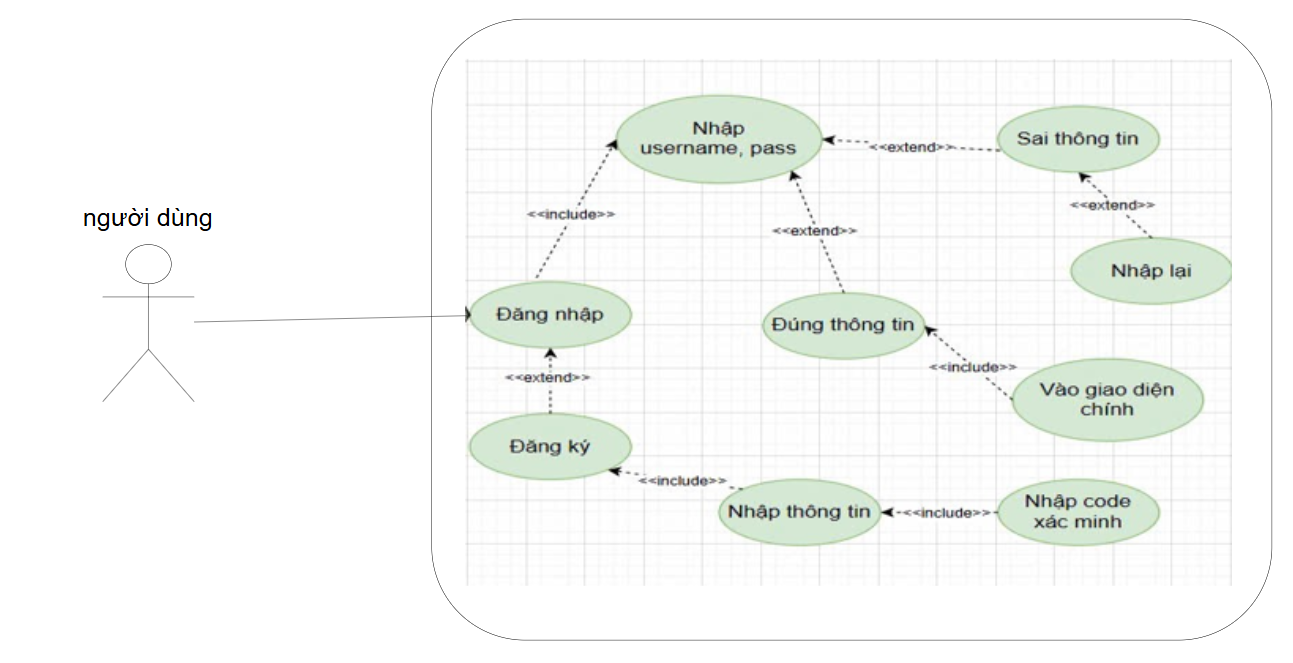
\includegraphics[width=0.8\textwidth]{useCaseDangNhap.png}

\clearpage

\subsubsection{Usecase quản lý note}
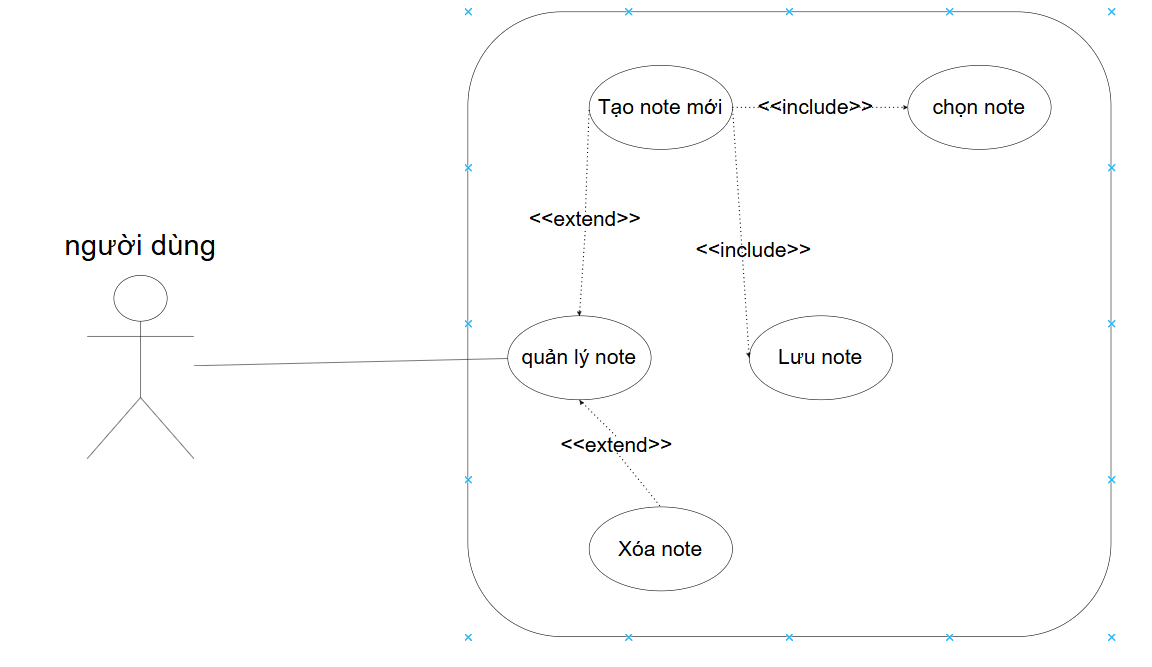
\includegraphics[width=0.8\textwidth]{useCasequanly.png}
\subsubsection{Usecase tìm kiếm và phân loại note}
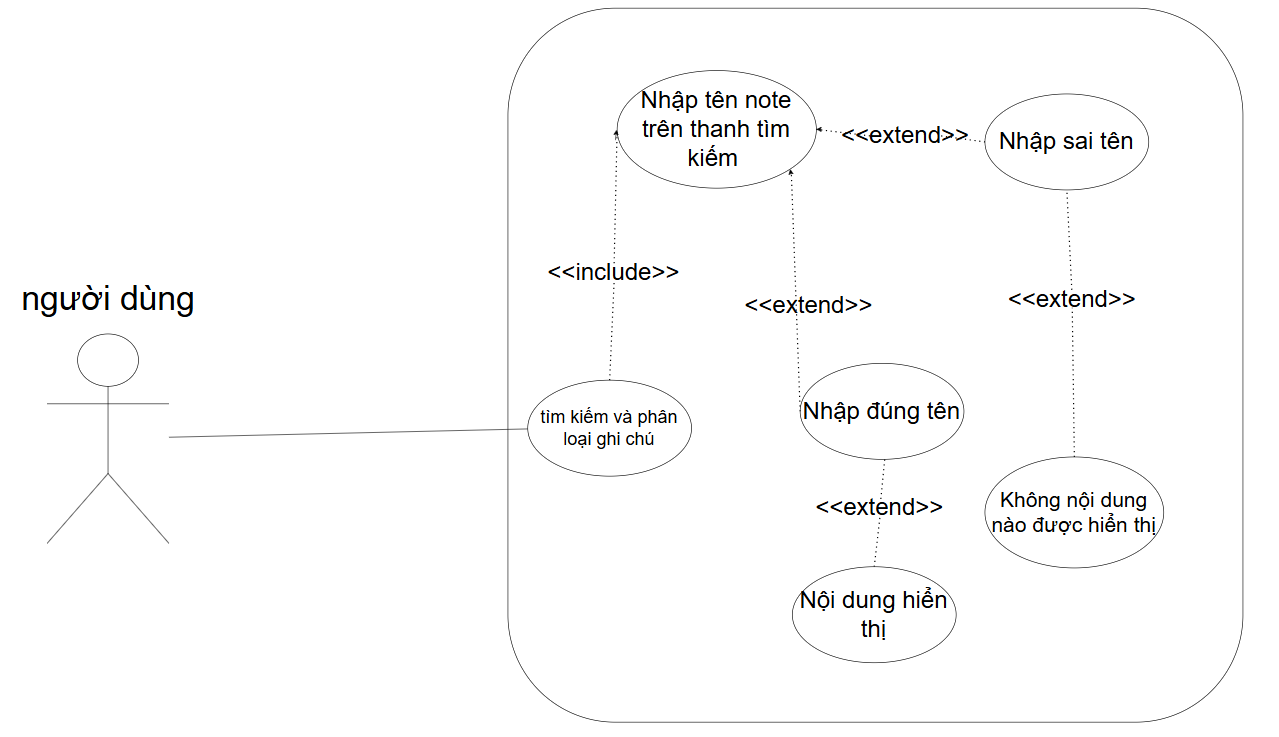
\includegraphics[width=0.8\textwidth]{useCasetimkiem.png}
\subsubsection{Use case hiển thị U/I}
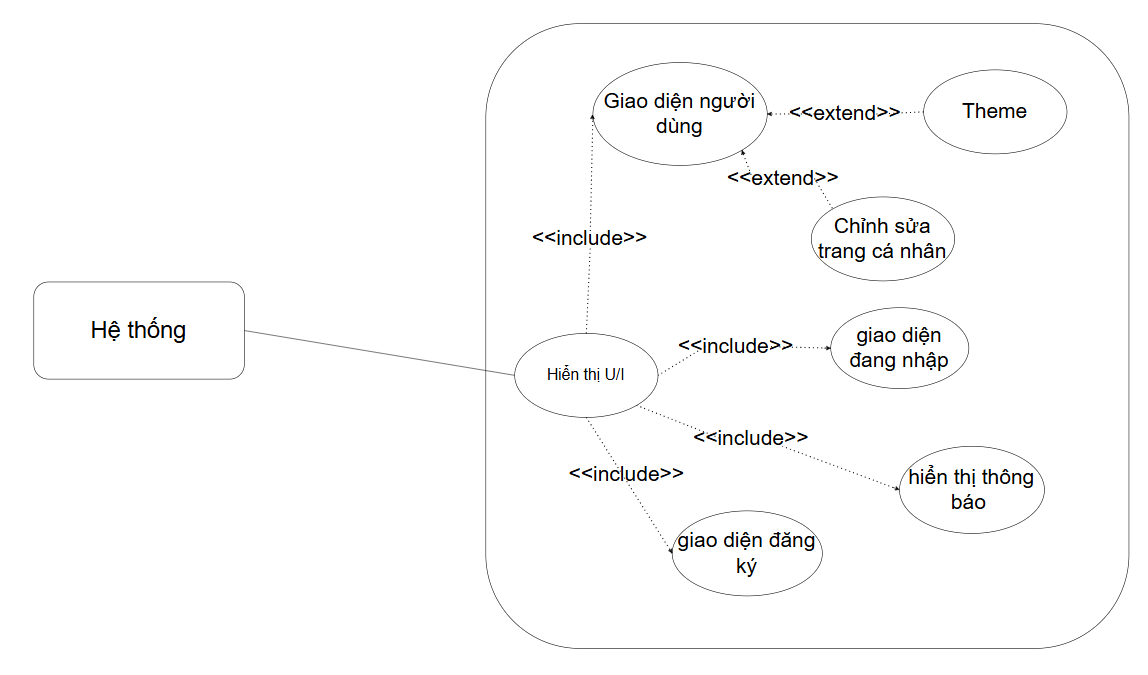
\includegraphics[width=0.8\textwidth]{useCaseUI.png}
\subsubsection{Usecase quản lý tài khoản cá nhân}
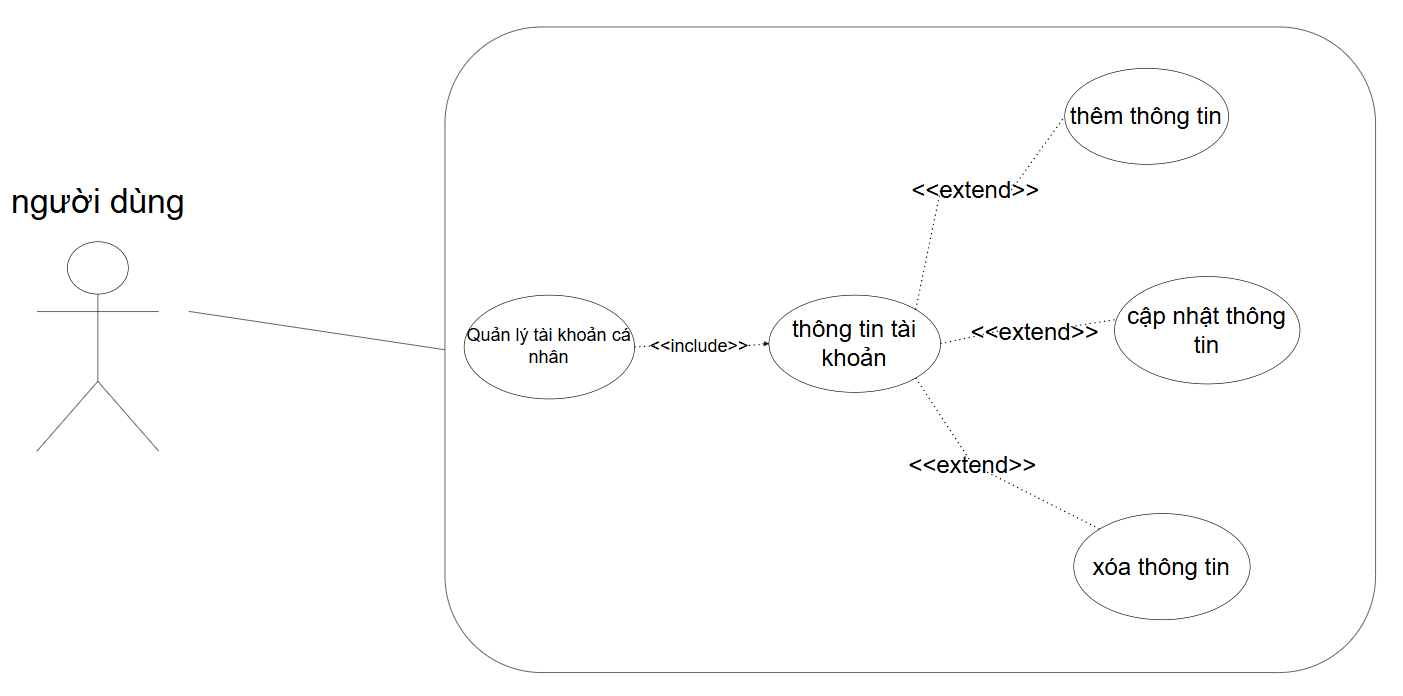
\includegraphics[width=0.8\textwidth]{useCasecanhan.png}

\subsection{Sơ đồ hoạt động (Activity Diagram)}
\subsubsection{Đặc tả UC-Đăng nhập}

\rowcolors{2}{white}{gray!10}
\begin{longtable}{|>{\raggedright\arraybackslash}p{4cm}|p{10cm}|}
\hline
\rowcolor{yellow!80!black} \multicolumn{2}{|c|}{\textbf{Use Case Description}} \\
\hline
\textbf{Use Case ID:} & UC-1 \\
\hline
\textbf{Tên:} & Hệ thống đăng nhập \\
\hline
\textbf{Mô tả:} & Xác thực danh tính người dùng \\
\hline
\textbf{Tiền điều kiện:} &
1. Đăng nhập: Có tài khoản hợp lệ, hệ thống hoạt động. \newline
2. Đăng ký: Chưa có tài khoản, cung cấp thông tin cá nhân, xác minh SĐT \& Email. \newline
3. Quên mật khẩu: Có tài khoản, nhập username \& SĐT, xác minh để đặt lại mật khẩu. \\
\hline
\textbf{Hậu điều kiện:} &
1. Đăng nhập: Thành công $\rightarrow$ vào hệ thống, thất bại $\rightarrow$ nhập lại hoặc quên mật khẩu. \newline
2. Đăng ký: Thành công $\rightarrow$ tài khoản mới, thất bại $\rightarrow$ nhập lại thông tin. \newline
3. Quên mật khẩu: Thành công $\rightarrow$ đặt mật khẩu mới, thất bại $\rightarrow$ thử lại hoặc hỗ trợ. \newline
Thoát: Kết thúc phiên, về giao diện đăng nhập. \\
\hline
\textbf{Luồng sự kiện chính:} &
1. Truy cập hệ thống $\rightarrow$ hiển thị giao diện đăng nhập. \newline
2. Đăng nhập: Nhập username/password $\rightarrow$ đúng vào hệ thống, sai yêu cầu nhập lại. \newline
3. Đăng ký: Nhập thông tin cá nhân $\rightarrow$ xác minh SĐT/email $\rightarrow$ đúng tạo tài khoản, sai nhập lại. \newline
4. Quên mật khẩu: Nhập username \& SĐT $\rightarrow$ xác minh $\rightarrow$ đúng đặt lại mật khẩu. \newline
5. Thoát: kết thúc phiên, quay lại giao diện đăng nhập. \\
\hline
\textbf{Luồng sự kiện phụ:} &
1. Nhập sai username/password $\rightarrow$ nhập lại, sai nhiều lần có thể khóa tạm thời. \newline
2. Sai mã xác minh $\rightarrow$ nhập lại, quá số lần giới hạn phải gửi lại mã. \newline
3. Thông tin đăng ký không hợp lệ $\rightarrow$ nhập lại. \newline
4. Không nhận mã xác minh $\rightarrow$ gửi lại hoặc xác minh bằng email. \newline
5. Người dùng có thể hủy/quay lại bất cứ lúc nào. \\
\hline
\end{longtable}

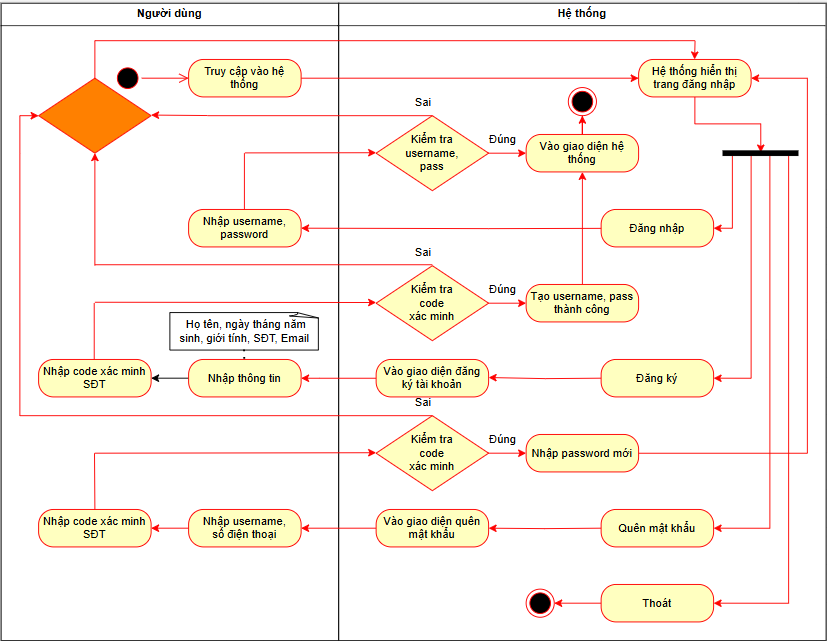
\includegraphics[width=0.8\textwidth]{UCdangnhap2.png}

\clearpage

\subsubsection{Đặc tả UC-Xóa note}
\rowcolors{2}{white}{gray!10}
\begin{longtable}{|>{\raggedright\arraybackslash}p{4cm}|p{10cm}|}
\hline
\rowcolor{yellow!80!black} \multicolumn{2}{|c|}{\textbf{Use Case Description}} \\
\hline
\textbf{Use Case ID:} & UC-2 \\
\hline
\textbf{Tên:} & Hệ thống xóa note \\
\hline
\textbf{Mô tả:} & Cho phép người dùng chọn và xóa note đã tạo. \\
\hline
\textbf{Tiền điều kiện:} &
1. Người dùng đã đăng nhập vào hệ thống. \newline
2. Người dùng đã có note trong hệ thống. \newline
3. Hệ thống hoạt động bình thường và có thể truy xuất note. \\
\hline
\textbf{Hậu điều kiện:} &
1. Nếu xóa note thành công $\rightarrow$ note bị xóa khỏi cơ sở dữ liệu. \newline
2. Nếu xóa note thất bại (do lỗi hệ thống hoặc người dùng không xác nhận) $\rightarrow$ note vẫn giữ nguyên. \\
\hline
\textbf{Luồng sự kiện chính:} &
1. Người dùng chọn chức năng “Xóa note”. \newline
2. Hệ thống hiển thị danh sách note đã tạo. \newline
3. Người dùng chọn note muốn xóa. \newline
4. Hệ thống yêu cầu xác nhận xóa note: \newline
\hspace*{1em}– Nếu người dùng xác nhận $\rightarrow$ note bị xóa khỏi CSDL. \newline
\hspace*{1em}– Nếu người dùng từ chối $\rightarrow$ Kết thúc quy trình. \\
\hline
\textbf{Luồng sự kiện phụ:} &
1. Người dùng không có note trong hệ thống $\rightarrow$ Hệ thống thông báo và không cho phép xóa. \newline
2. Người dùng nhập sai hoặc chọn nhầm note $\rightarrow$ Có thể quay lại để chọn lại. \newline
3. Hệ thống gặp lỗi khi xóa note $\rightarrow$ Hiển thị thông báo lỗi, yêu cầu thử lại sau. \newline
4. Người dùng thay đổi ý định sau khi chọn note $\rightarrow$ Có thể quay lại mà không xóa. \\
\hline
\end{longtable}
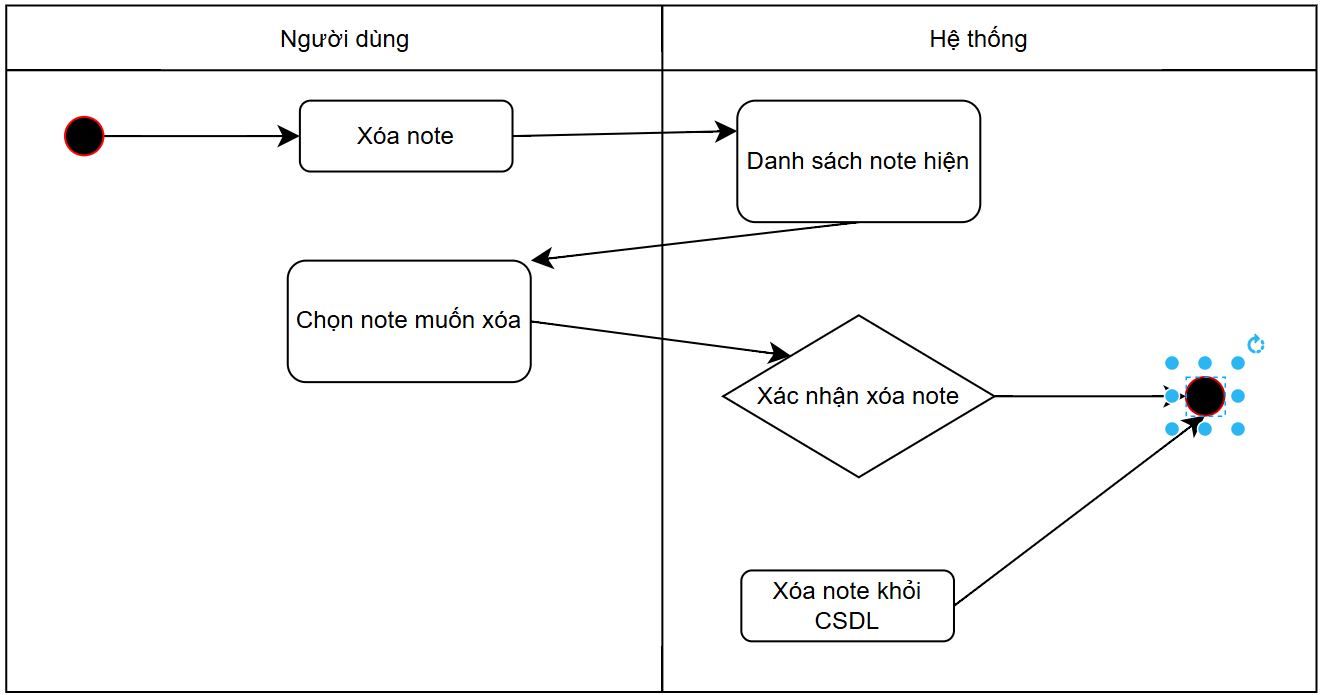
\includegraphics[width=0.8\textwidth]{UCxoanote.png}

\clearpage

\subsubsection{Đặc tả UC-Tạo Note}
\rowcolors{2}{white}{gray!10}
\begin{longtable}{|>{\raggedright\arraybackslash}p{4cm}|p{10cm}|}
\hline
\rowcolor{yellow!80!black} \multicolumn{2}{|c|}{\textbf{Use Case Description}} \\
\hline
\textbf{Use Case ID:} & UC-3 \\
\hline
\textbf{Tên:} & Hệ thống tạo note \\
\hline
\textbf{Mô tả:} & Quy trình tạo note của hệ thống \\
\hline
\textbf{Tiền điều kiện:} &
1. Người dùng đã đăng nhập vào hệ thống. \newline
2. CSDL chứa các thông tin cần thiết hiện có. \\
\hline
\textbf{Hậu điều kiện:} &
1. Người dùng đã tạo note thành công và thông tin giao dịch được lưu vào cơ sở dữ liệu. \newline
2. Hệ thống thông báo cho người dùng (thành công hoặc thất bại). \\
\hline
\textbf{Luồng sự kiện chính:} &
1. Người dùng nhấn vào nút “Tạo ghi chú” (+). \newline
2. Hệ thống hiển thị giao diện nhập ghi chú. \newline
3. Người dùng nhập tiêu đề và nội dung ghi chú. \newline
4. Người dùng nhấn nút “Lưu”. \newline
5. Hệ thống kiểm tra dữ liệu đầu vào. \newline
6. Hệ thống lưu ghi chú vào cơ sở dữ liệu cục bộ. \newline
7. Hệ thống hiển thị thông báo “Lưu thành công” và quay lại danh sách ghi chú. \\
\hline
\textbf{Luồng sự kiện phụ:} &
1. Hệ thống thông báo “Vui lòng nhập nội dung hoặc tiêu đề.” \newline
2. Quay lại bước 3. \\
\hline
\end{longtable}
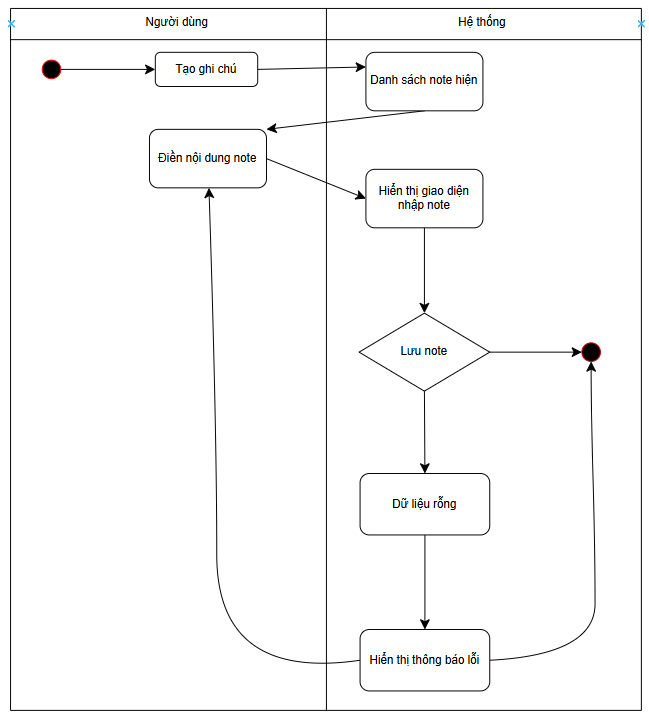
\includegraphics[width=0.8\textwidth]{UCtaonote.png}
\subsubsection{Đặc tả UC - Xem note}
\rowcolors{2}{white}{gray!10}
\begin{longtable}{|>{\raggedright\arraybackslash}p{4cm}|p{10cm}|}
\hline
\rowcolor{yellow!80!black} \multicolumn{2}{|c|}{\textbf{Use Case Description}} \\
\hline
\textbf{Use Case ID:} & UC-4 \\
\hline
\textbf{Tên:} & Hệ thống xem note \\
\hline
\textbf{Mô tả:} & Cho phép người dùng tra cứu note của mình \\
\hline
\textbf{Tiền điều kiện:} &
1. Người dùng đã đăng nhập vào hệ thống. \newline
2. Hệ thống có dữ liệu về note mà người dùng đã nhập. \\
\hline
\textbf{Hậu điều kiện:} &
1. Hiển thị thông tin note của người dùng theo yêu cầu. \newline
2. Nếu người dùng muốn xem thêm ngày tháng chi tiết hơn, hệ thống tiếp tục thực hiện truy vấn. \newline
3. Nếu không có thao tác tiếp theo, quy trình kết thúc. \\
\hline
\textbf{Luồng sự kiện chính:} &
1. Người dùng chọn chức năng “Xem chi tiết”. \newline
2. Hệ thống sẽ hiển thị ra chi tiết ngày tháng đó. \newline
3. Người dùng bấm thêm lần nữa để kết thúc hành động. \\
\hline
\textbf{Luồng sự kiện phụ:} &
\textbf{Trường hợp:} \newline
1. Danh sách ghi chú rỗng: \newline
- Người dùng mở ứng dụng. \newline
- Hệ thống phát hiện danh sách ghi chú rỗng. \newline
- Hệ thống hiển thị thông báo: “Chưa có ghi chú nào. Nhấn thêm để tạo mới”. \newline
2. Ghi chú đã bị xóa hoặc không còn tồn tại: \newline
- Người dùng chọn ghi chú từ danh sách. \newline
- Hệ thống không tìm thấy dữ liệu ghi chú. \newline
- Hệ thống hiển thị thông báo lỗi: “Ghi chú không tồn tại hoặc bị xóa”. \\
\hline
\end{longtable}
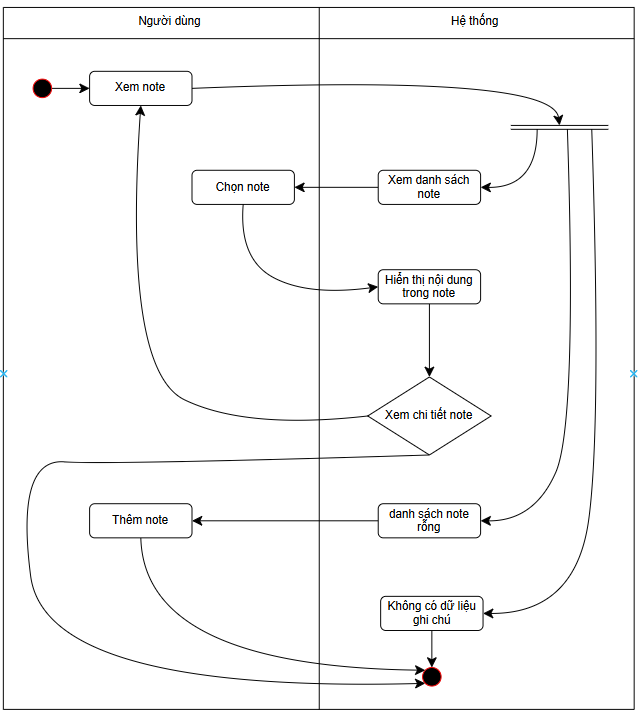
\includegraphics[width=0.8\textwidth]{UCxemnote.png}

\clearpage
\subsubsection{Đặc tả UC-Thêm thông tin người dùng }
\rowcolors{2}{white}{gray!10}
\begin{longtable}{|>{\raggedright\arraybackslash}p{4cm}|p{10cm}|}
\hline
\rowcolor{yellow!80!black} \multicolumn{2}{|c|}{\textbf{Use Case Description}} \\
\hline
\textbf{Use Case ID:} & UC-5 \\
\hline
\textbf{Tên:} & Hệ thống thêm thông tin người dùng \\
\hline
\textbf{Mô tả:} & Thêm thông tin người dùng \\
\hline
\textbf{Tiền điều kiện:} &
Người dùng có quyền điều chỉnh thông tin của mình \\
\hline
\textbf{Hậu điều kiện:} &
1. Người dùng thêm thông tin vào biểu mẫu đăng ký. \newline
2. Hệ thống nhận thông tin người dùng mà người dùng nhập vào bao gồm: ID, username, ngày tháng năm sinh, giới tính, SĐT, email. \\
\hline
\textbf{Luồng sự kiện chính:} &
1. Người dùng truy cập mục “Thông tin cá nhân” từ giao diện chính hoặc menu cài đặt. \newline
2. Hệ thống hiển thị biểu mẫu nhập thông tin (ví dụ: tên, email, mô tả cá nhân...). \newline
3. Người dùng nhập hoặc cập nhật thông tin. \newline
4. Người dùng nhấn nút Lưu. \newline
5. Hệ thống kiểm tra tính hợp lệ của dữ liệu đầu vào. \newline
6. Nếu hợp lệ, hệ thống lưu thông tin vào cơ sở dữ liệu. \newline
7. Hệ thống hiển thị thông báo “Cập nhật thành công”. \\
\hline
\textbf{Luồng sự kiện phụ:} &
\textbf{Trường hợp:} \newline
1. Thiếu thông tin bắt buộc: \newline
- Hệ thống sẽ yêu cầu nhập đầy đủ thông tin. \newline
2. Dữ liệu sai: \newline
- Dữ liệu nhập vào sai. \newline
- Lỗi khi lưu. \newline
- Cập nhật thất bại. \\
\hline
\end{longtable}
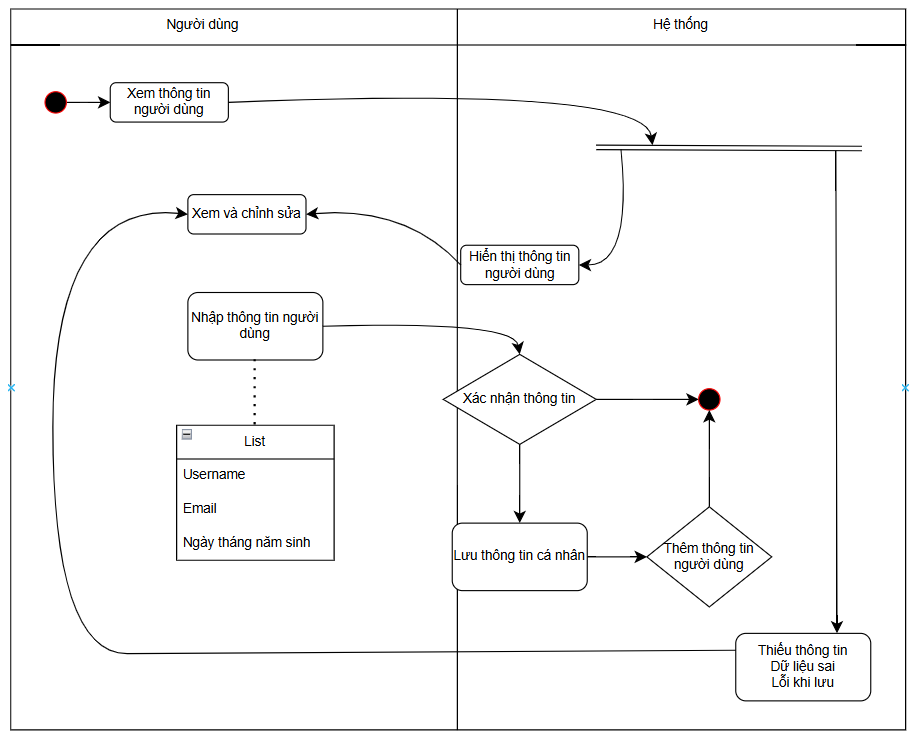
\includegraphics[width=0.7\textwidth]{UCthongtin.png}

\clearpage
\subsection{Sơ đồ tuần tự (Sequence Diagram}
\subsubsection{Sơ đồ tuần tự đăng nhập}
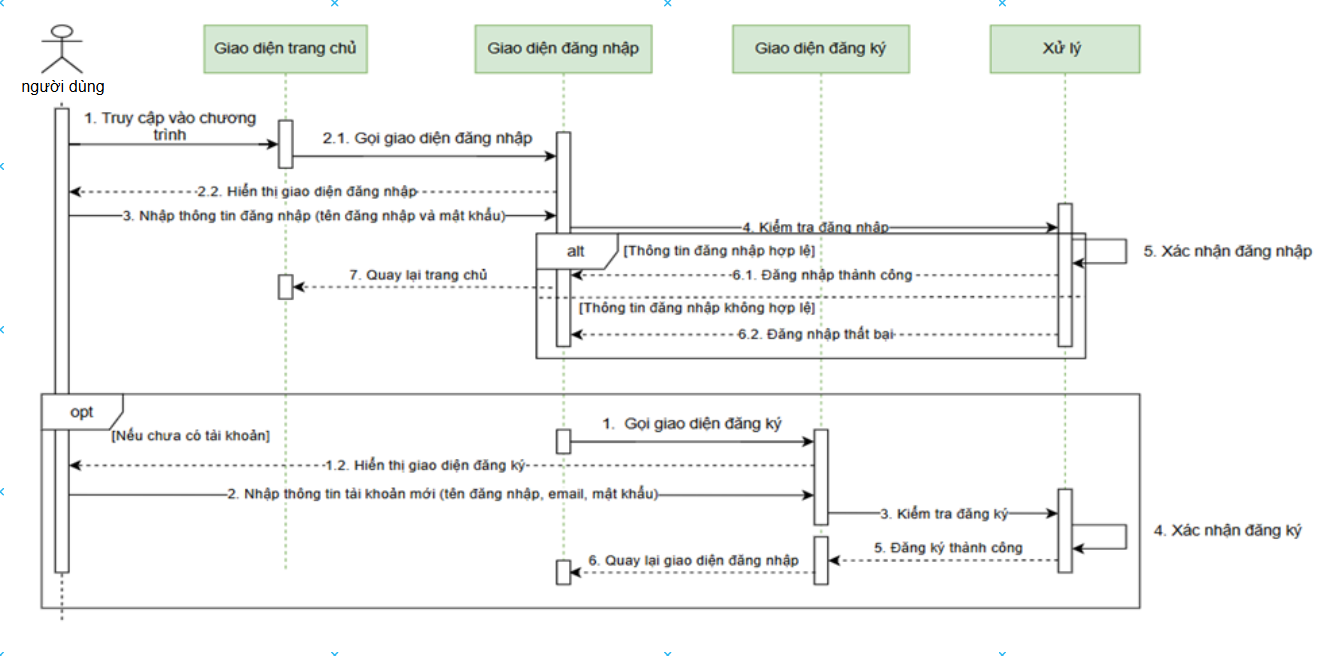
\includegraphics[width=0.8\textwidth]{SDdangnhap.png}
\subsubsection{Sơ đồ tuần tự tạo note}
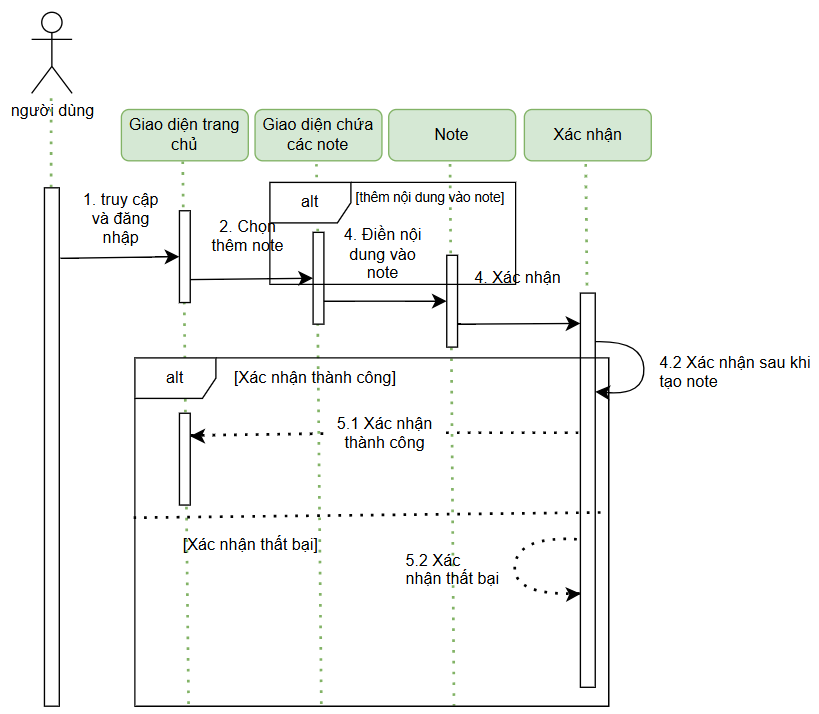
\includegraphics[width=0.8\textwidth]{SDtaonote.png}

\clearpage

\subsubsection{Sơ đồ tuần tự chỉnh sửa note}
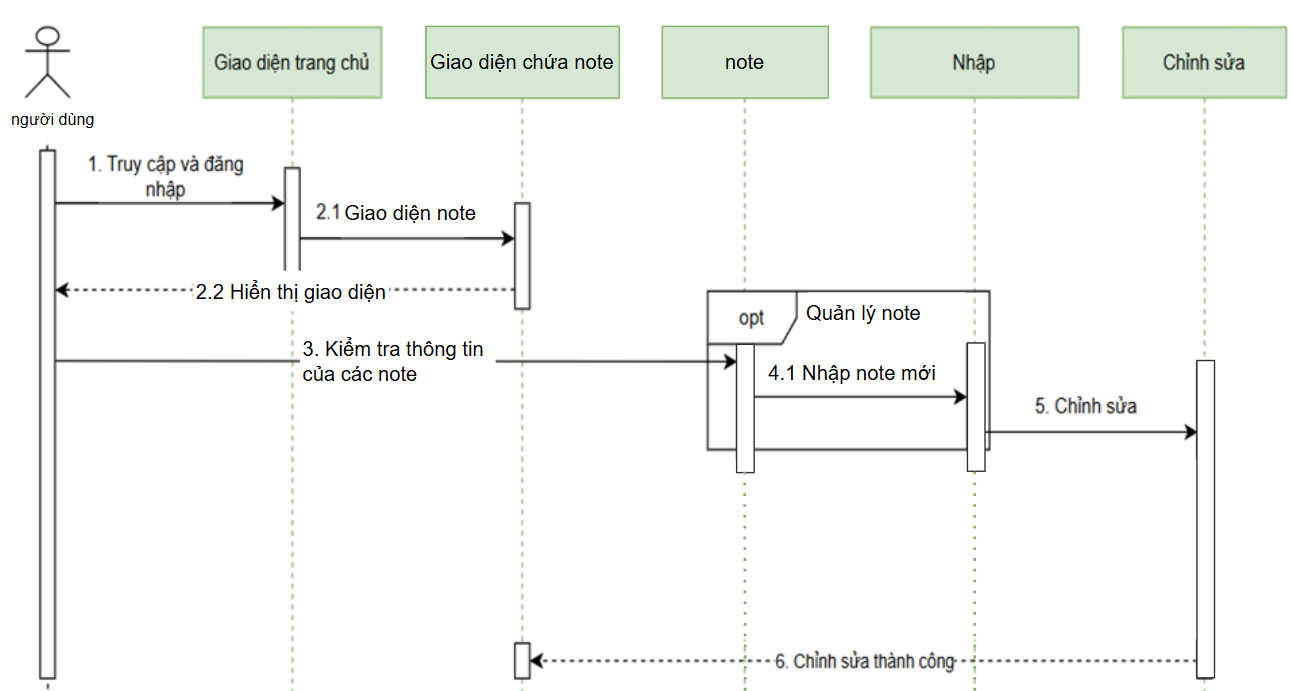
\includegraphics[width=0.8\textwidth]{SDsuanote.png}
\subsubsection{Sơ đồ tuần tự note}
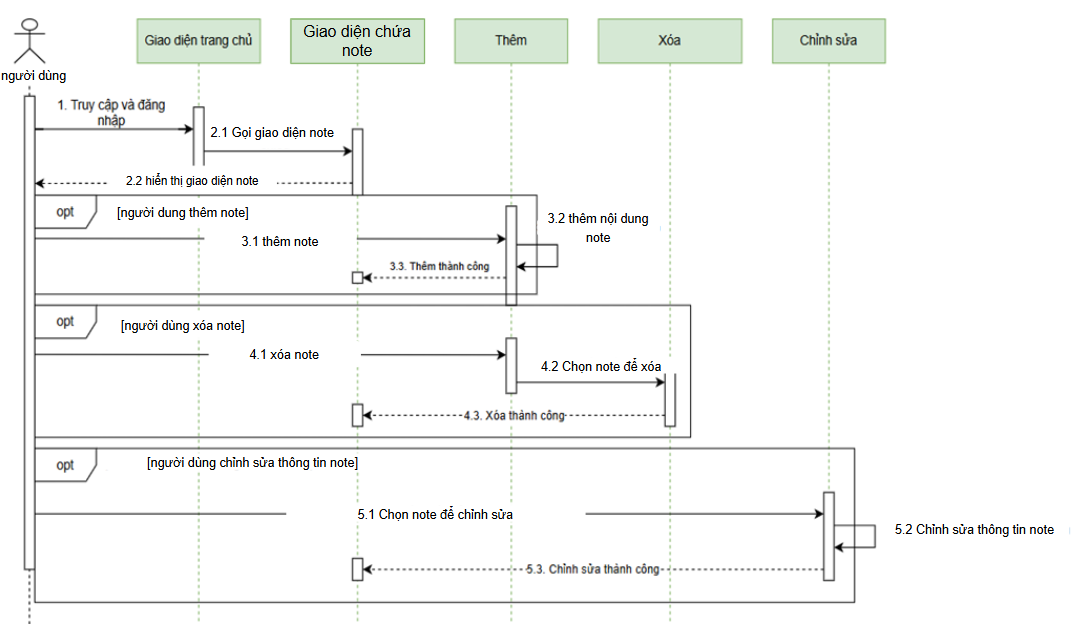
\includegraphics[width=0.8\textwidth]{SDtuantu.png}

\clearpage
\section{THIẾT KẾ GIAO DIỆN HỆ THỐNG}
\subsection{Sơ đồ menu chính}
\begin{center}
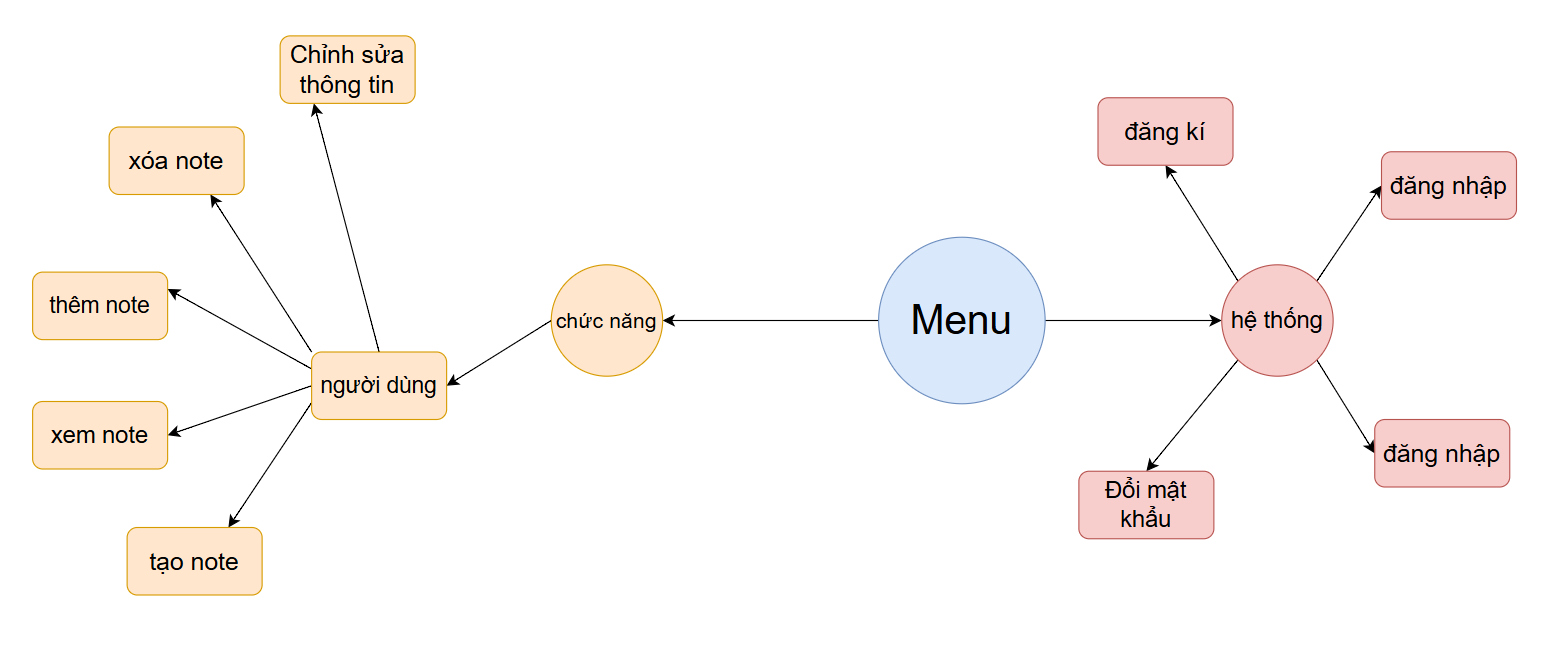
\includegraphics[width=0.8\textwidth]{SDmenuchinh.png}
\end{center}
Phần này trình bày sơ đồ tư duy (mind map) thể hiện cấu trúc chức năng chính của ứng dụng \textbf{TakeNote}, với trung tâm là mục ``\textbf{Menu}''. Sơ đồ được chia thành hai nhánh chính, mỗi nhánh đại diện cho một nhóm chức năng khác nhau mà người dùng có thể sử dụng. Cụ thể:

\begin{itemize}
    \item \textbf{Menu} (trung tâm, màu xanh lam): Đây là điểm chính của giao diện người dùng, từ đây có thể điều hướng đến các chức năng khác nhau của hệ thống.
    
    \item \textbf{Chức năng} (nhánh màu vàng nhạt, bên trái): Nhánh này liên kết với ``Người dùng'' và bao gồm các chức năng chỉnh sửa, thêm, xóa, xem và tạo ghi chú. Cụ thể:
    \begin{itemize}
        \item \textbf{Chỉnh sửa thông tin}: Người dùng có thể chỉnh sửa thông tin cá nhân như tên, email, mô tả.
        \item \textbf{Xóa note}: Cho phép người dùng xóa các ghi chú không cần thiết.
        \item \textbf{Thêm note}: Tạo ghi chú mới.
        \item \textbf{Xem note}: Hiển thị danh sách các ghi chú đã tạo.
        \item \textbf{Tạo note}: Tạo mới ghi chú từ đầu.
    \end{itemize}
    
    \item \textbf{Hệ thống} (nhánh màu hồng nhạt, bên phải): Nhánh này bao gồm các chức năng liên quan đến tài khoản người dùng, bao gồm:
    \begin{itemize}
        \item \textbf{Đăng ký}: Tạo tài khoản mới.
        \item \textbf{Đăng nhập}: Đăng nhập vào hệ thống.
        \item \textbf{Đổi mật khẩu}: Thay đổi mật khẩu hiện tại.
    \end{itemize}
\end{itemize}

Sơ đồ này giúp mô tả cách mà ứng dụng \textbf{TakeNote} tổ chức các chức năng chính, giúp người dùng dễ dàng hình dung luồng tương tác và hoạt động của hệ thống một cách hiệu quả và trực quan.

\clearpage
\subsection{Thiết kế giao diện}
\subsubsection{Giao diện trang chủ}
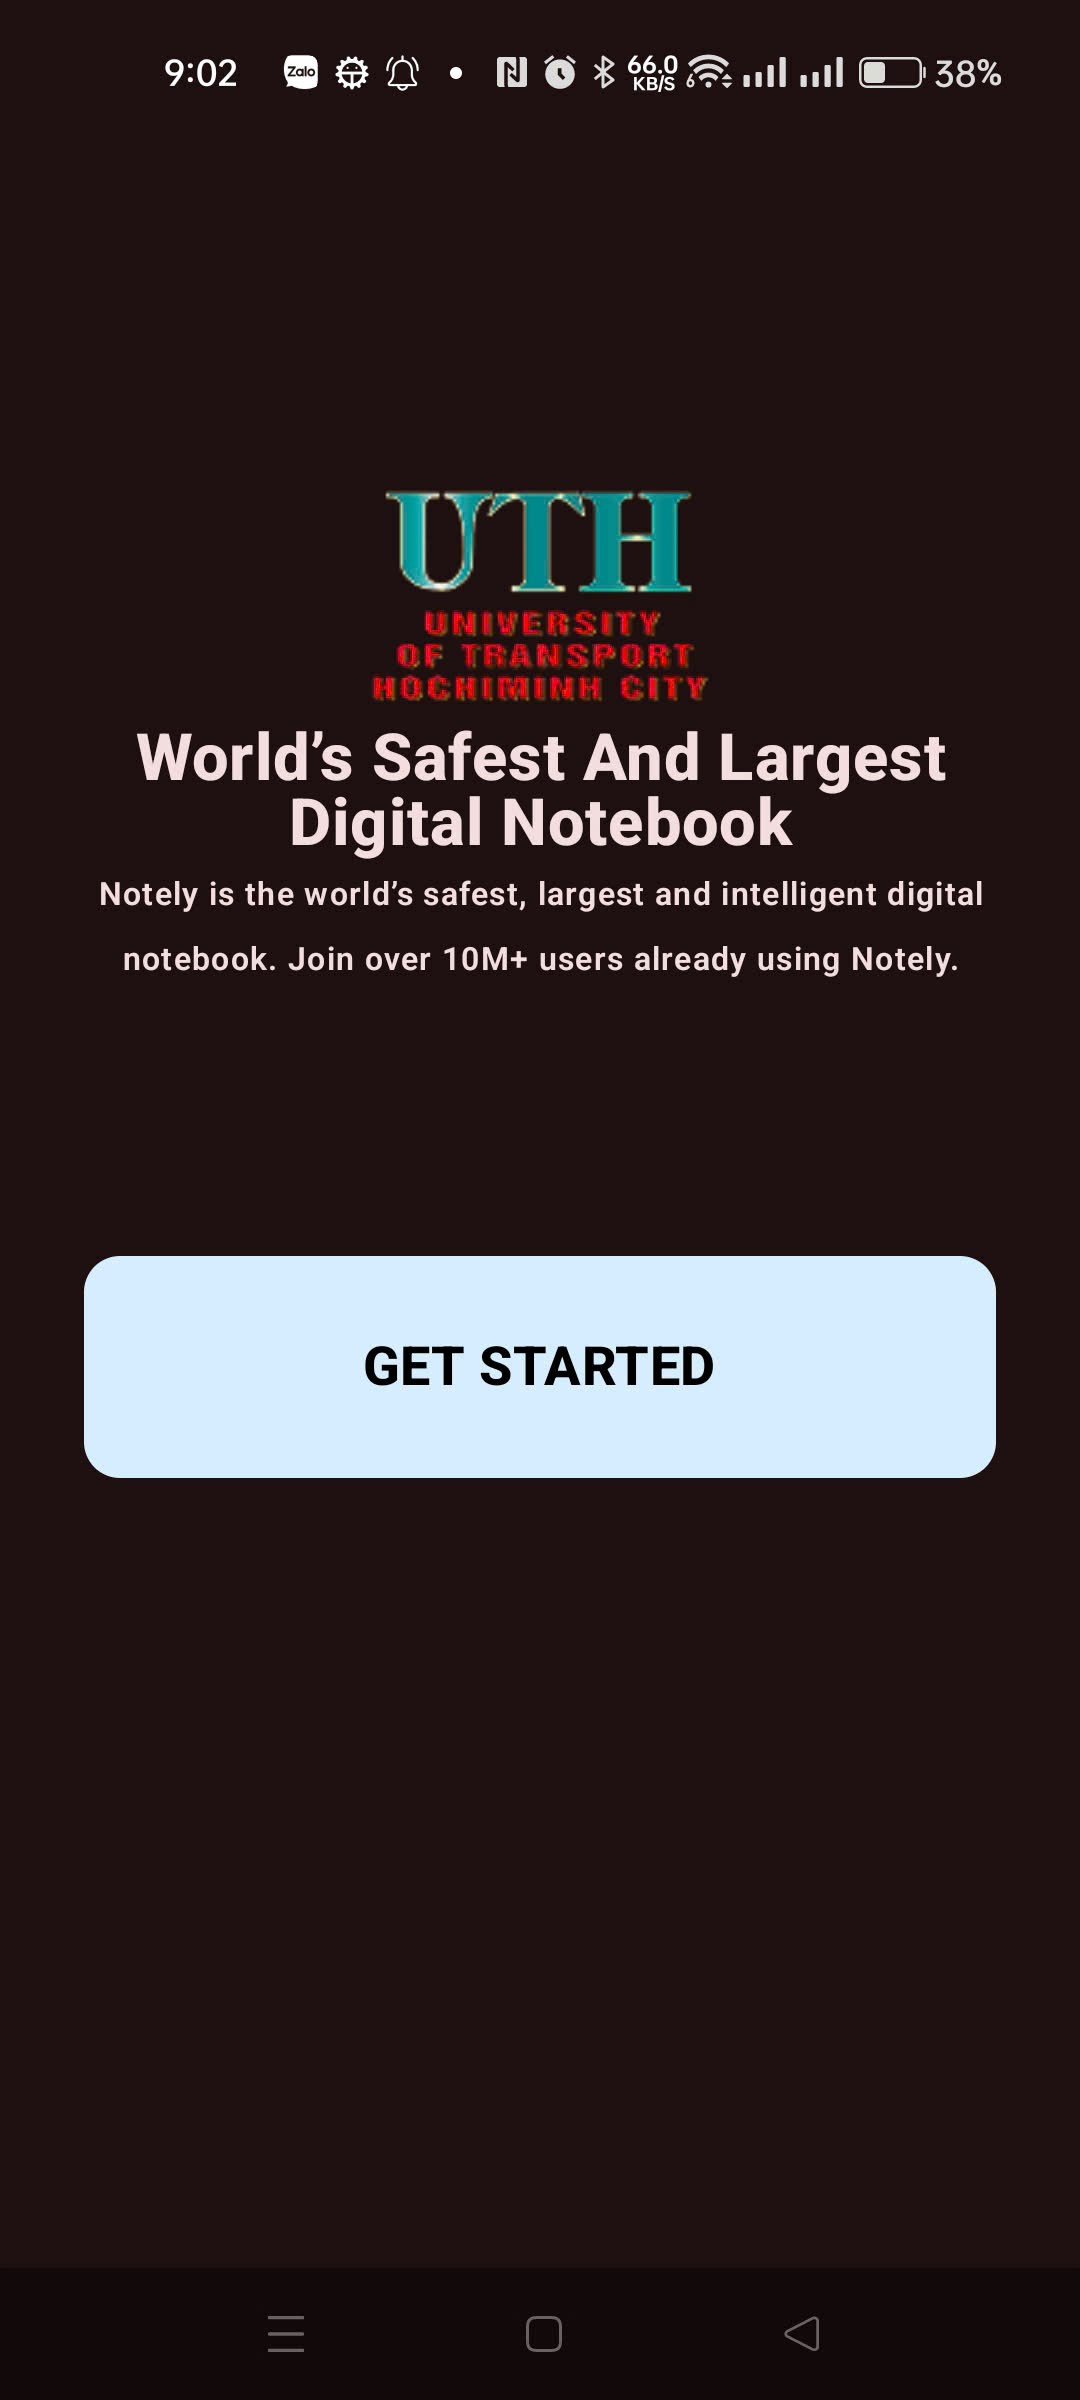
\includegraphics[width=0.6\textwidth]{GiaoDien.png}
\clearpage
\subsubsection{Giao diện đăng nhập bằng google}

\includegraphics[width=0.6\textwidth]{GiaoDienDangNhap.png}
\clearpage
\subsubsection{Giao diện chứa note}
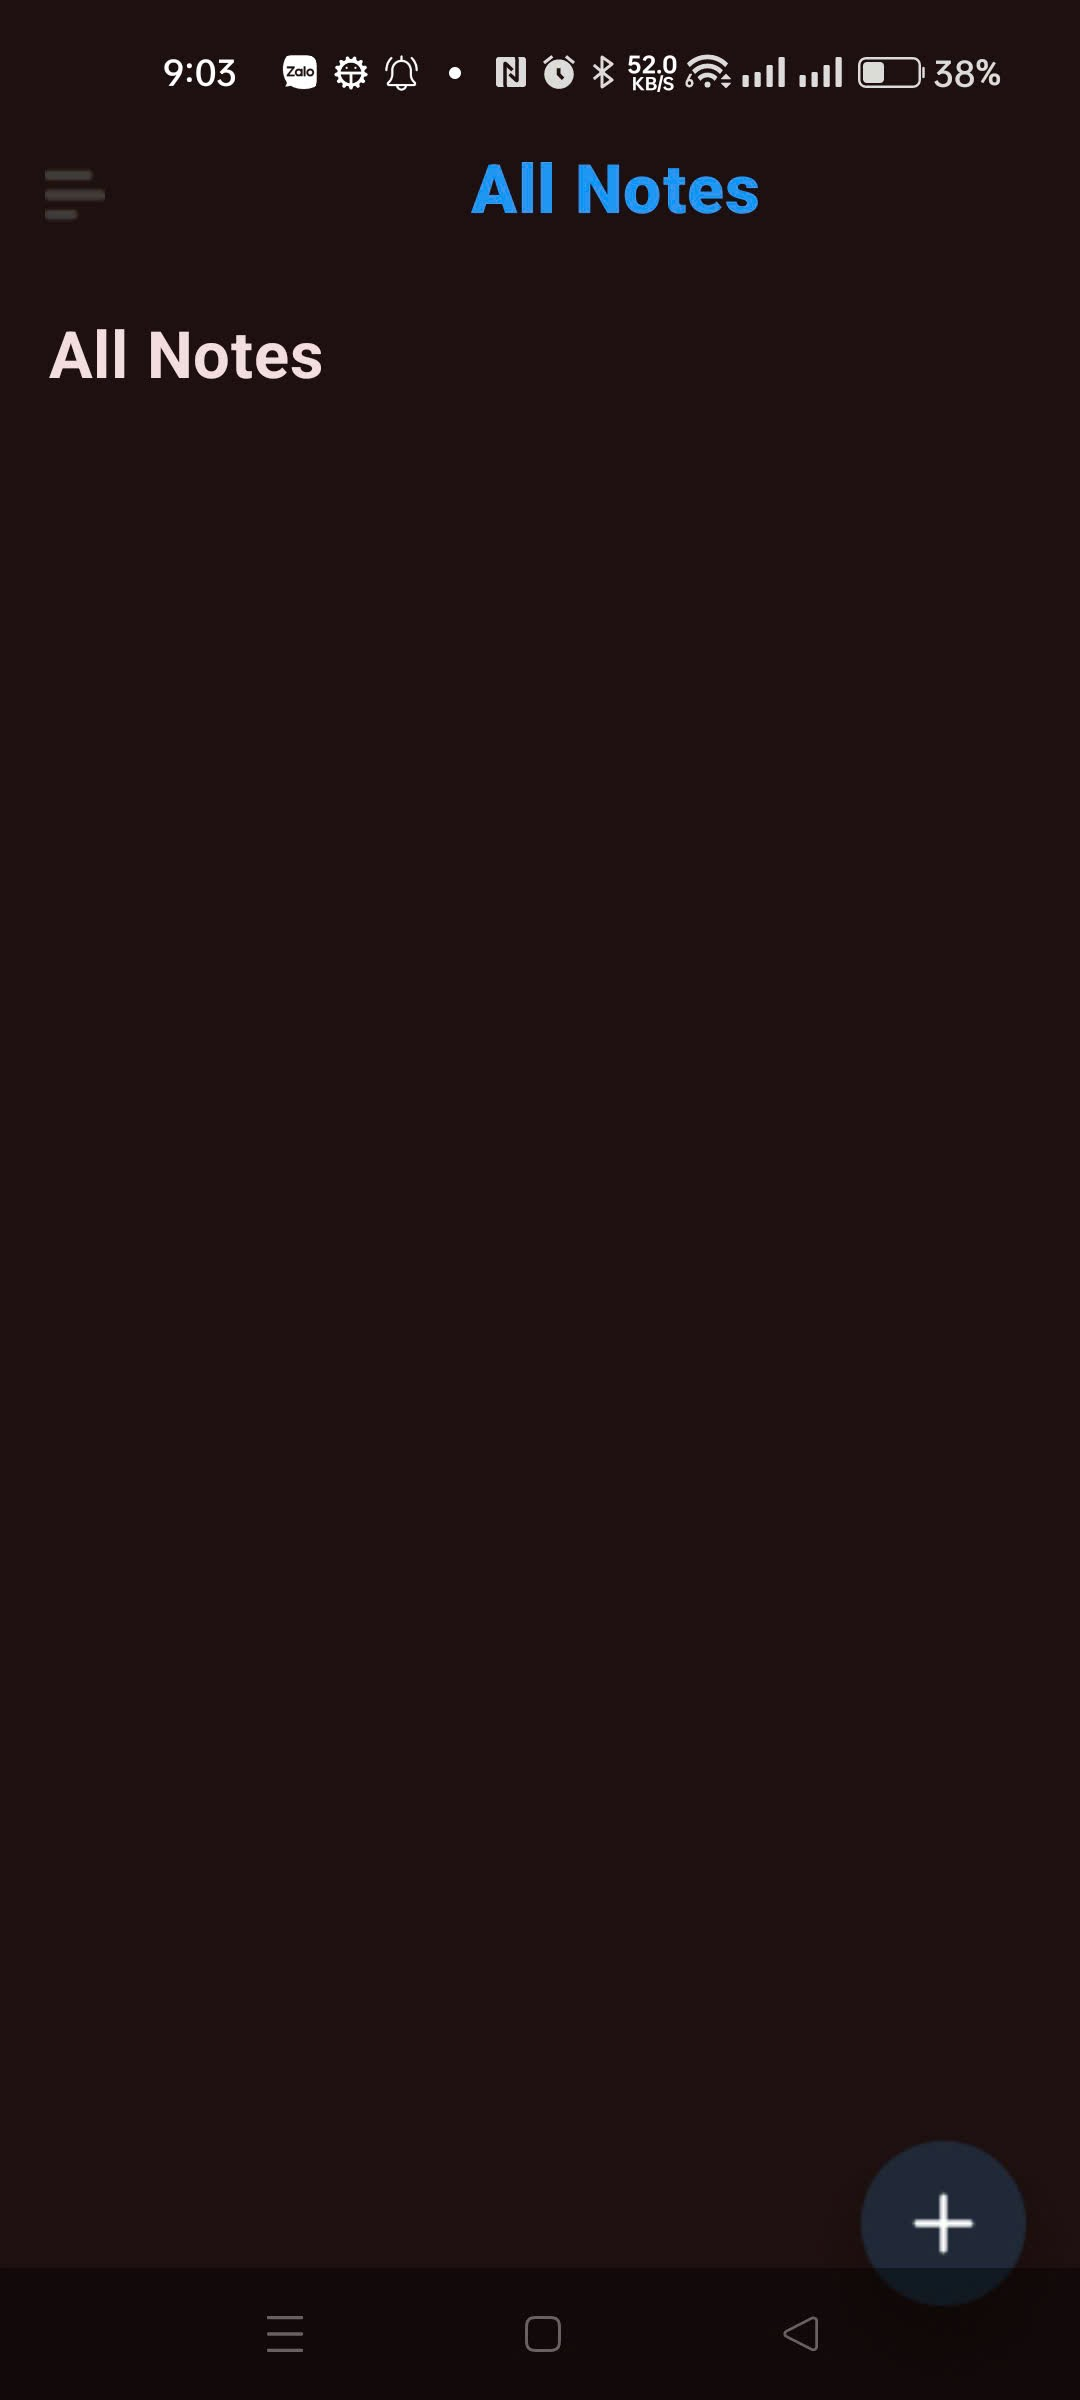
\includegraphics[width=0.6\textwidth]{GiaoDienChuanote.png}
\clearpage
\subsubsection{Giao diện điền note}
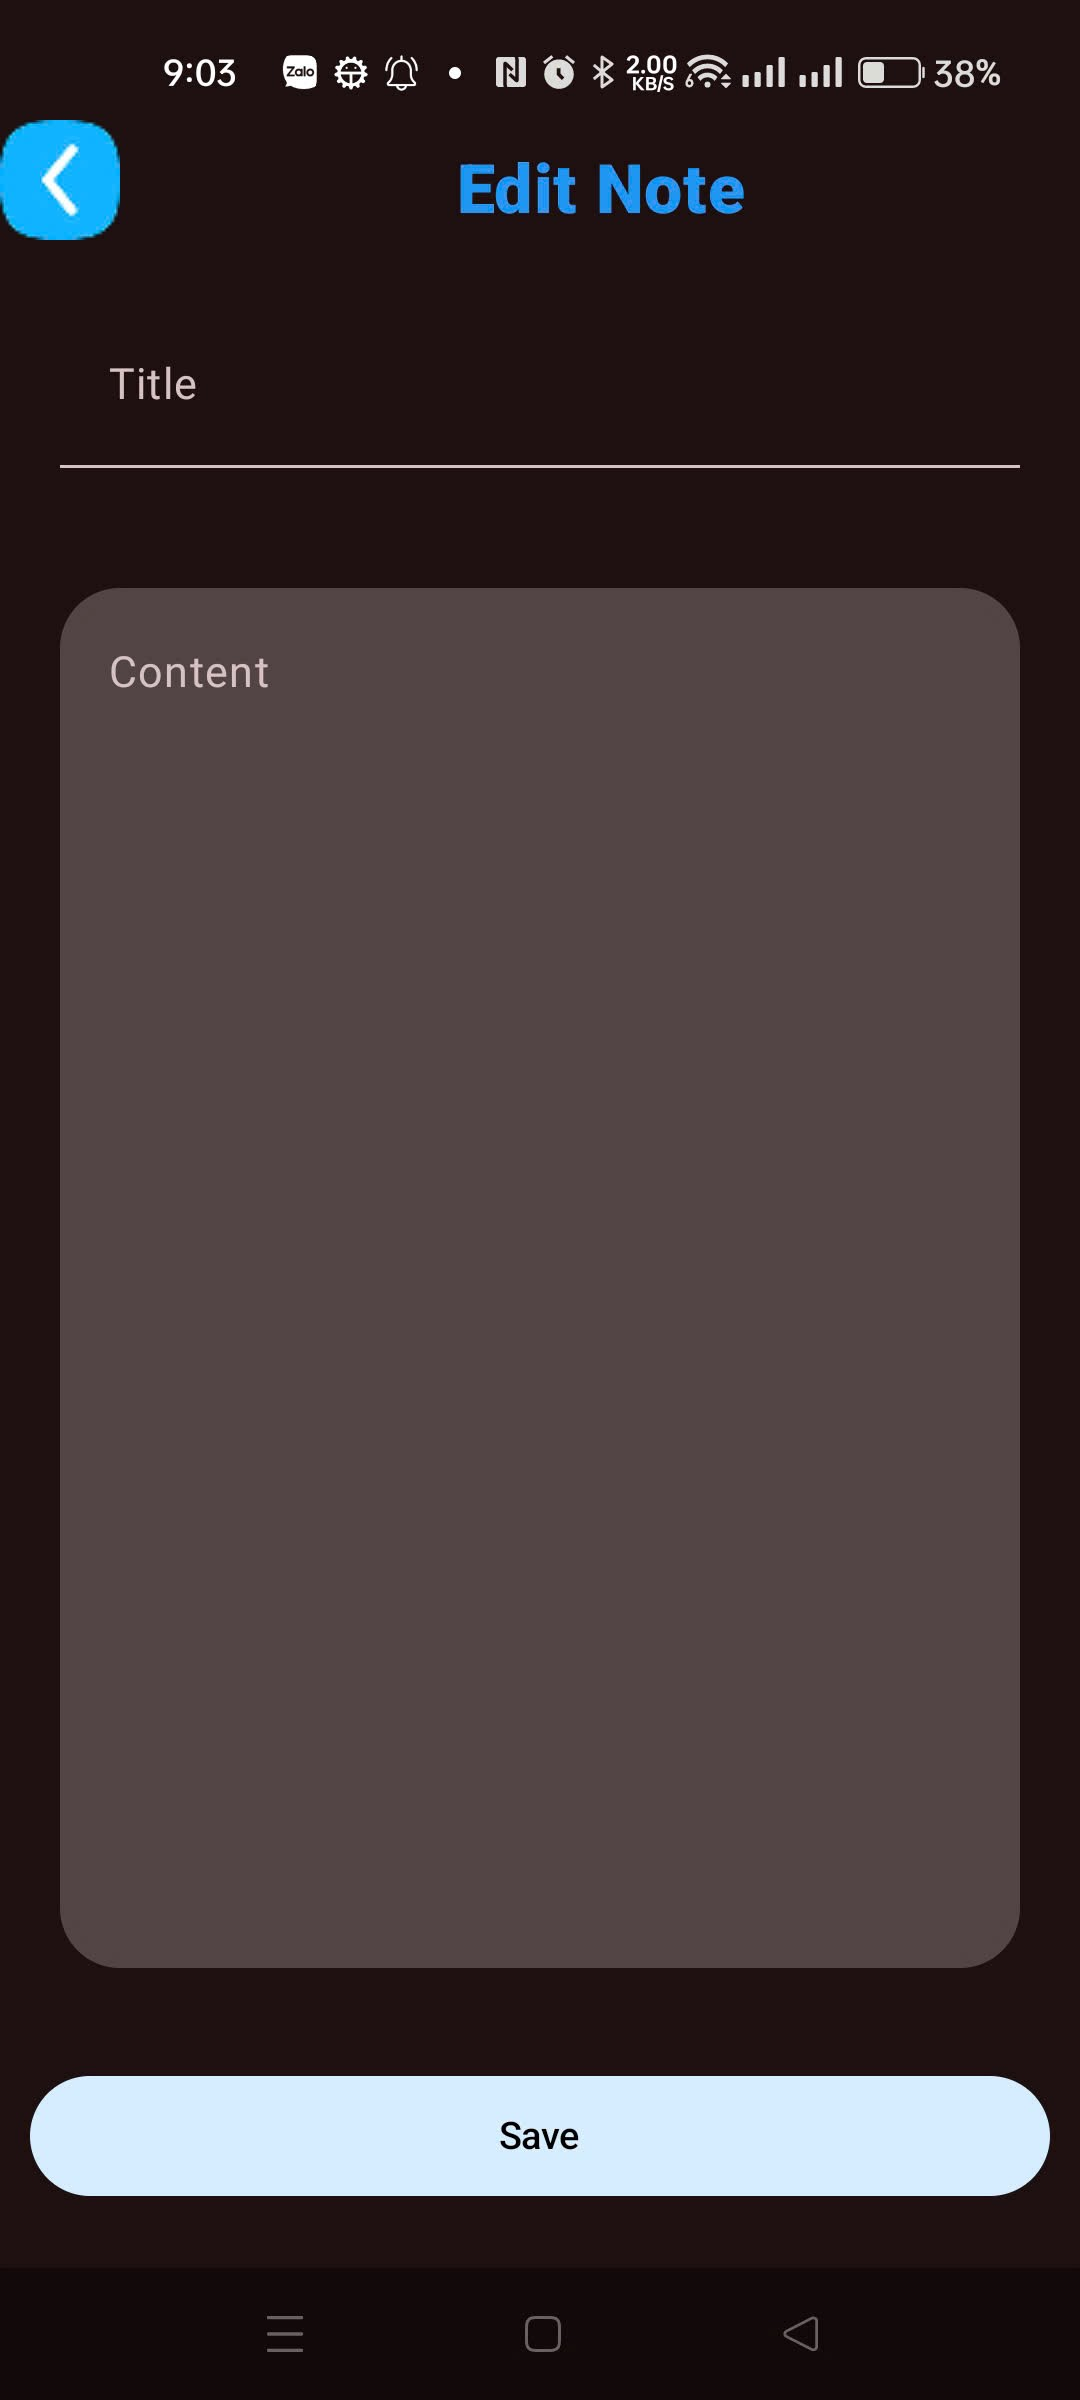
\includegraphics[width=0.6\textwidth]{GiaoDiendiennote.png}
\clearpage
\subsubsection{Giao diện profile}
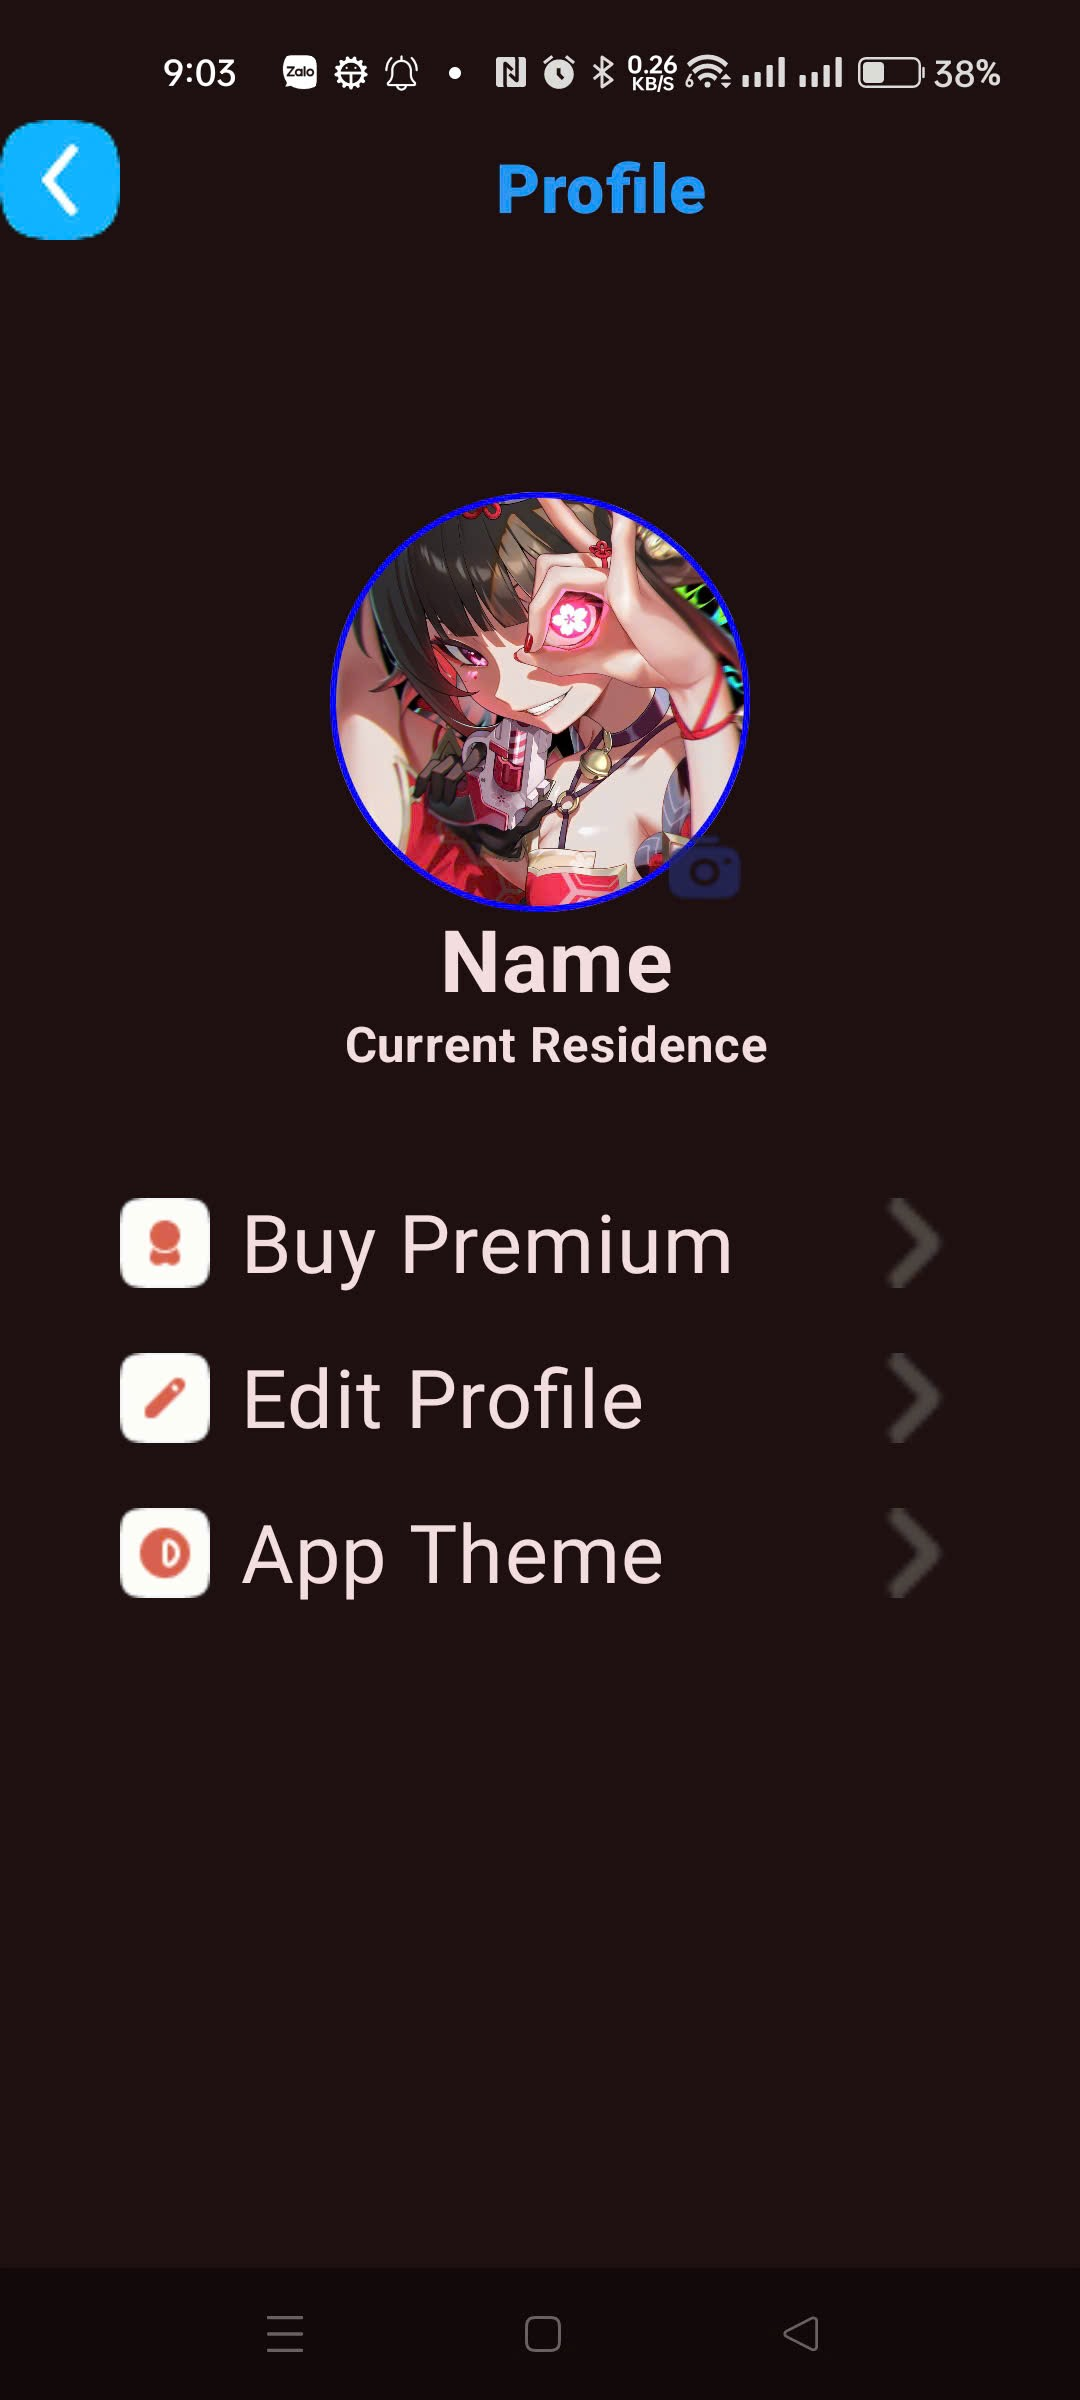
\includegraphics[width=0.6\textwidth]{profile.png}

\clearpage
\section{TỔNG KẾT}
\subsection{Kết quả đạt được}
Ứng dụng \textbf{TakeNote} giúp tối ưu hoá ghi chú, tự động hoá quản lý ghi chú, ý tưởng, tài liệu và nội dung số. Hệ thống cải thiện trải nghiệm người dùng, giảm sai sót, tiết kiệm thời gian và nâng cao hiệu quả công việc.

\subsection{Đánh giá ưu, khuyết điểm}

\subsubsection{Ưu điểm}
\begin{itemize}
    \item Cải thiện trải nghiệm người dùng: Giao diện mượt mà, trực quan giúp người dùng dễ dàng thao tác và truy cập tài liệu.
    \item Bảo mật cao: Nhờ vào việc sao lưu được tài khoản Google để đăng nhập giúp giảm thiểu các trường hợp đánh mất dữ liệu.
    \item Dễ mở rộng: Hỗ trợ tích hợp nhiều tính năng nâng cao.
\end{itemize}

\subsubsection{Khuyết điểm}
\begin{itemize}
    \item Yêu cầu bảo mật cao: Cần biện pháp mạnh mẽ để bảo vệ dữ liệu.
    \item Bù trừ mô tông: Còn 1 vài chức năng như đổi \textit{theme}, mua sắm nội dung để nâng cao dung lượng lưu trữ, lưu thông tin cá nhân chưa được phát triển 1 cách đầy đủ.
    \item Rủi ro kỹ thuật: Có thể có lỗi trong quá trình đưa ứng dụng đến vận hành.
\end{itemize}

\subsection{Hướng phát triển tương lai}
\begin{itemize}
    \item Tích hợp AI để giúp người dùng trong việc sắp xếp dữ liệu một cách ngay lập tức.
    \item Có thể lưu trữ dữ liệu lớn trong 1 thời gian dài nhờ nâng cao bảo mật cấp độ lưu trữ.
\end{itemize}

\subsection{Kết luận}
Hệ thống app \textbf{TakeNote} hiện tại đã đáp ứng tốt nhu cầu người dùng về việc tạo các note nhanh, lưu trữ tài liệu an toàn. Việc tiếp tục phát triển công nghệ này sẽ giúp hệ thống ngày càng hoàn thiện và phù hợp với định hướng thực tế hiện nay.

\end{document}
